\section{Introduction to the Problem}
Let the \emph{height} of a ladder be the number of rows that a ladder has with at least one bar. 
Let $MinL\{\pi\} \subseteq OptL\{\pi\}$ such that the ladders in $MinL\{\pi\}$ are the ladders of shortest height from 
$OptL\{\pi\}$.  Let \emph{a minimal ladder} be a ladder from $MinL\{\pi\}$. The \emph{Minimum Height Problem} asks, 
given a permutation $\pi$, is there an algorithm for creating a minimal ladder
from $MinL\{\pi\}$?\par  
Two tangential questions that result from this problem are the following. Let $MinL\{\pi_{n}\}$ 
be the set of all $MinL\{\pi\}$ for each permutation of order $n$. Recall that $OptL\{\pi_{n}\}$ is the set of all 
$OptL\{\pi\}$ of order $n$. Thus, $MinL\{\pi_{n}\} \subseteq OptL\{\pi_{n}\}$.  The first tangential question is, 
what are the upper and lower bounds for the heights of ladders in $MinL\{\pi_{n}\}$? 
Let \emph{ladders of order n} pertain to ladders derived from some $\pi$ with $n$ elements.
The second tangential question is what ladders of order $n$ have a height of zero or one? \par 


I will address the tangential questions in the introduction. Following the tangential questions, 
I will provide a number of algorithms for generating one ladder from $MinL\{\pi\}$ in the procedures section; one 
of which is a heuristic algorithm. 
In the results section I will provide a table with the heights of the ladder from the heuristic 
algorithm in comparison to the heights of the ladders
in $MinL\{\pi\}$. Finally, in the analysis section there will be a discussion 
about the efficacy of the heuristic algorithm along with some applications of the algorithm.\par 


%%Upper and lower bounds question
\subsection{Upper and Lower Bounds of the heights of the Ladders in each $MinL\{\pi_{n}\}$}
In this section the upper and lower bounds for the heights of the ladders in $MinL\{\pi_{n}\}$ will be determined;
not the upper and lower bounds for the heights of the ladders in $OptL\{\pi_{n}\}$. Seeing as $MinL\{\pi_{n}\}\subseteq OptL\{\pi_{n}\}$, 
by determining the lower bound for the height of $MinL\{\pi_{n}\}$, the lower bound for the height of $OptL\{\pi_{n}\}$ will also be determined. 
\begin{lemma}
    The lower bound for the height of a ladder $MinL\{\pi_{n}\}$ is zero
\end{lemma} 
\begin{proof}
    If $\pi_{n}$ is the sorted permutation of order $n$ then there are no 
    bars in its ladder. Recall that a bar swaps an adjacent inversion in $\pi$.
    Seeing as there are no adjacent inversions in the sorted permutation of 
    order $n$, then there are no bars that need to be added to its corresponding 
    ladder. Since a ladder with no bars requires no rows, then the lower 
    bound for the height of a ladder from $MinL{\pi_{n}}$ is zero. 
\end{proof}\par 
The upper bound for the heights of the ladders in $MinL\{\pi_{n}\}$ is more difficult to prove than the lower bound. 
The lower bound is unique seeing as there is only one ladder of order $n$ with zero bars. 
With the upper bound however, it has yet to be shown if there is an upper bound for 
$MinL\{\pi_{n}\}$. Before proving the upper bound for $MinL\{\pi_{n}\}$ it must be shown how to 
derive the ladder with minimal height from the root ladder of the reverse permutation of order $n$.
Refer to this ladder as $MinL(Rev(\pi_{n}))$.
Once we have established how to derive $MinL(Rev(\pi_{n}))$ from the root ladder 
of the reverse permutation of order $n$, it will be relatively easy to prove the upper bound 
for $MinL\{\pi_{n}\}$.\par 
 Let $Rev(\pi_{n})$ be the reverse permutation of order 
 $n$.
 Let $RootL(Rev(\pi_{n}))$ be the root ladder for $Rev(\pi_{n})$. Recall that the root ladder is the ladder such 
    that no bar of a lesser element has crossed the route of a greater element. $RootL(Rev(\pi_{n}))$ requires 
    $2(n-1)-1$ rows. See theorem~\ref{Theorem:One}.\par 
   
   In order to create $MinL(Rev(\pi_{n}))$, one simply needs to 
   take $RootL(Rev(\pi_{n}))$ and modify it. In order to modify $RootL(Rev(\pi_{n}))$ correctly, consider what happens when 
   the bars of lesser elements are right swapped above the routes of greater elements. Of course, if this is done to $RootL(Rev(\pi_{n}))$ then 
   the ladder is no longer $RootL(Rev(\pi_{n}))$. Nonetheless, when the $n-1th$ route is swapped above the $nth$ route, 
   this frees up an extra row in the ladder for the $n-2th$ route. This is the row where the last bar of the $n-1th$ element resided
   before it was swapped above the $nth$ route. Now, the first bar of the $n-1th$ route will begin in column $2$ and end at column $n-1$. 
   Furthermore, a new row will need to be added to the top of the ladder in order to accommodate the first bar of the $n-1th$ route. Now the route 
   of the $n-2th$ element can be raised up a row seeing as its last bar will still be in column $n-3$ and the row/column 
   that was previously occupied by the last bar of the $n-1th$ element will be free. Then the $n-3$ route can be swapped above 
   the route of elements $n-2 \dots n$. The route of $n-3$ will begin at column $4$ and span to column $n-1$. 
   Since a new row was already added above route $n$ for element $n-1$, 
   the first bar of element $n-3$ begins at the 
   same row as the first bar for element $n-1$. By swapping 
   all the $n-jth$, $1 \leq J < (n-1)$ and $j=2k+1$, routes above the routes of elements 
   $(n-j)+1 \dots n$ in $RootL(Rev(\pi_{n}))$, the ladder is reconfigured to $MinL(Rev(\pi_{n}))$. The height of $MinL(Rev(\pi_{n}))$ is $n$ 
   because the $nth$ element still requires $n-1$ rows, and the $n-1th$ element requires one additional row to be added above 
   the row for the first bar of the $nth$ element. Please refer 
   to Figure \ref{Fig:RootToMinLadder} for an example of modifying $RootL(5,4,3,2,1)$ to $MinL(5,4,3,2,1)$.
   Now that $MinL(Rev(\pi))$ has been established, we can prove the upper bound for
   $MinL\{\pi_{n}\}$.  
   %%Please refer to Algorithm \ref{Alg:MinRevLadder} to see the algorithm for creating $MinL(Rev(\pi_{n}))$ irrespective of $RootL(Rev(\pi_{n}))$.\pagebreak

    \begin{center}
        \begin{figure}[!htp]
            \begin{minipage}{.4\textwidth}
                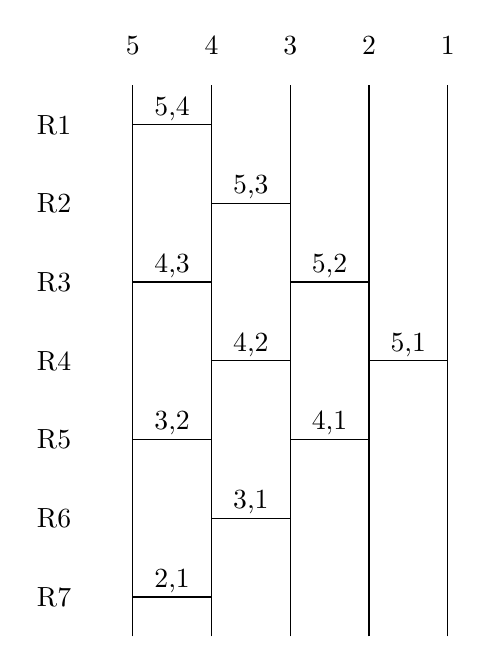
\begin{tikzpicture}
                    \draw(0, -1) to (0, 6);
                        %%draw the bars
                        \draw(0, 5.5) to (1, 5.5);
                            \node at (.5, 5.7){5,4};
                        \draw(0, 3.5) to (1, 3.5);
                            \node at (.5, 3.7){4,3};
                        \draw(0, 1.5) to (1, 1.5);
                            \node at (.5, 1.7){3,2};
                        \draw(0, -.5) to (1, -.5);
                            \node at (.5, -.3){2,1};
                    \draw(1, -1) to (1, 6);
                        \draw(1, 4.5) to (2, 4.5);
                            \node at(1.5, 4.7){5,3};
                        \draw(1, 2.5) to (2, 2.5);
                            \node at (1.5, 2.7){4,2};
                        \draw(1, .5) to (2, .5);
                            \node at(1.5, .7){3,1};
                    \draw(2, -1) to (2, 6);
                        \draw(2, 3.5) to (3, 3.5);
                            \node at(2.5, 3.7){5,2};
                        \draw(2, 1.5) to (3, 1.5);
                            \node at(2.5, 1.7){4,1};
                    \draw(3, -1) to (3, 6);
                        \draw(3, 2.5) to (4, 2.5);
                            \node at (3.5, 2.7){5,1};
                    \draw(4, -1) to (4, 6);

                    %%draw the rows
                    \node at (-1, 5.5){R1};
                    \node at(-1, 4.5){R2};
                    \node at(-1, 3.5){R3};
                    \node at (-1, 2.5){R4};
                    \node at(-1, 1.5){R5};
                    \node at (-1, 0.5){R6};
                    \node at (-1, -.5){R7};
                    %%draw the elements above the columns
                    \node at (0, 6.5){5};
                    \node at (1, 6.5){4};
                    \node at (2, 6.5){3};
                    \node at (3, 6.5){2};
                    \node at (4, 6.5){1};
                \end{tikzpicture}
            \end{minipage}
            \hfill
             \begin{minipage}{.4\textwidth}
                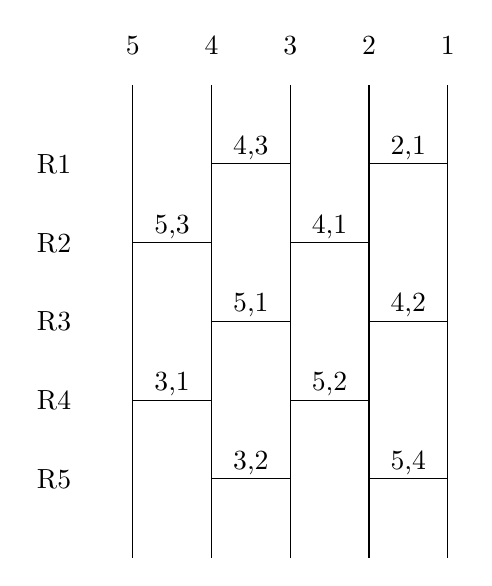
\begin{tikzpicture}
                    \draw(0, 0) to (0, 6);
                        \draw(0, 4) to (1, 4);
                            \node at(.5, 4.2){5,3};
                        \draw(0, 2) to (1, 2);
                            \node at(.5, 2.2){3,1};
                    \draw(1, 0) to (1, 6);
                        \draw(1, 3) to (2, 3);
                            \node at(1.5, 3.2){5,1};
                        \draw(1, 5) to (2, 5);
                            \node at(1.5, 5.2){4,3};
                        \draw(1, 1) to (2, 1);
                            \node at(1.5, 1.2){3,2};
                    \draw(2, 0) to (2, 6);
                        \draw(2, 2) to (3, 2);
                            \node at(2.5, 2.2){5,2};
                        \draw(2, 4) to (3, 4);
                            \node at(2.5, 4.2){4,1};
                    \draw(3, 0) to (3, 6);
                        \draw(3, 1) to (4, 1);
                            \node at(3.5, 1.2){5,4};
                        \draw(3, 3) to (4, 3);
                            \node at(3.5, 3.2){4,2};
                        \draw(3, 5) to (4, 5);
                            \node at(3.5, 5.2){2,1};
                    \draw(4, 0) to (4, 6);


                    %%nodes above
                    \node at (0, 6.5){5};
                    \node at (1, 6.5){4};
                    \node at (2, 6.5){3};
                    \node at (3, 6.5){2};
                    \node at (4, 6.5){1};

                    %%rows
                    \node at (-1, 5){R1};
                    \node at (-1, 4){R2};
                    \node at (-1, 3){R3};
                    \node at (-1, 2){R4};
                    \node at (-1, 1){R5};

                    %%nodes
    
                \end{tikzpicture}
            \end{minipage}
            \caption{The ladder to the left is $Root(5,4,3,2,1)$. The ladder to the left is $MinL(5,4,3,2,1)$. Note that $n=5=2K+1$, thus 
            by swapping routes $2$ and $4$ above route $5$ whilst leaving route $3$ below route $5$ in $Root(5,4,3,2,1)$, we get 
            $MinL(5,4,3,2,1)$. There is no way to reduce the height further seeing as route $5$ still needs 
            $4$ rows and route $4$ needs one extra row for its first bar.}
            \label{Fig:RootToMinLadder}
        \end{figure}   

   \end{center}
   
   \begin{lemma}
       The upper bound for $MinL\{\pi_{n}\}$ is $n$.
   \end{lemma}
   \begin{proof}
       We shall use a proof by contradiction. Suppose that the upper bound for the height of $MinL\{\pi_{n}\}$ was greater than $n$. (It cannot be less than $n$ because 
       we have already demonstrated that the minimal height of the ladder for the reverse permutation is $n$). Let $MinL(Rev(n))$ be the 
       minimal ladder for the reverse permutation of order $n$. Refer to Figure~\ref{Fig:RootToMinLadder} for an example of $MinL(5,4,3,2,1)$. 
       It will be shown that for each permutation of order $n$, one of its minimal ladders can be derived from $MinL(Rev(n))$.
       Recall that a bar uninverts an inversion in a permutation. By removing bars from $MinL(Rev(n))$, that is effectively removing 
       inversions from $Rev(\pi(n))$. Of course, when a bar is removed from  $MinL(Rev(n))$, the ladder ceases to be $MinL(Rev(n))$. 
       Let $k$ be the number of bars in the current state of the ladder, with $MinL(Rev(n))$, $k=(n(n-1))/2$. For each subsequent 
       ladder, $0 \leq k < (n(n-1))/2$. Thus, to create the minimal ladders with $k=((n(n-1))/2)-1$ bars, 
       simply remove one of the correct bars from $MinL(Rev(n))$. 
       Once all the minimal ladders with  $k=((n(n-1))/2)-1$ bars have been created, simply remove the correct bar from each of these ladders with 
        $k=(n(n-1))/2-1$ bars to get all minimal ladders with  $k=((n(n-1))/2)-2$ bars.
       This process continues until each minimal ladder of order $n$ has been created. 
       Since bars are only being removed from ladders, no more rows 
       will be added to the ladder. 
       Removing a bar does not necessarily remove a row, but removing a bar definitely does not add a row to the ladder. 
       Earlier we stated that 
       the height of $MinL(Rev(n))$ is $n$, and at the same time we stated that we could create one minimal ladder order $n$ 
       from each $MinL\{\pi\}$ of order $n$
       by deriving it from $MinL(Rev(n))$ 
       through removing bars. Yet at the beginning of the proof, 
       we supposed the upper bound was greater than $n$ which contradicts the claim that by removing bars from  
       $MinL(Rev(n))$ the height of $MinL(Rev(n))$ will not increase. Thus, the upper bound for $MinL_\{\pi_{n}\}$ is $n$. 
       Please refer to Figure~\ref{Fig:RemovalSequence} for the removal sequence which lists $MinL\{\pi_{4}\}$. 

   \end{proof}\pagebreak

        \begin{figure}[!htp]
            \centering
            %%L1
            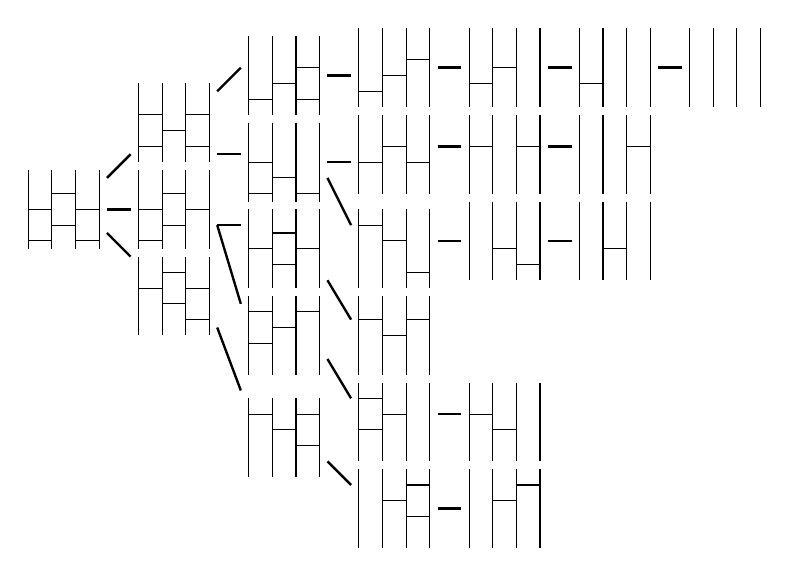
\begin{tikzpicture}
                \draw(0, -50) to (0, -51);
                    \draw(0, -50.5) to (.3, -50.5);
                    \draw(0, -50.9) to (.3, -50.9);
                \draw(0.3, -50) to (0.3, -51);
                    \draw(.3, -50.3) to (.6, -50.3);
                    \draw(.3, -50.7) to (.6, -50.7);
                \draw(0.6, -50) to (0.6, -51);
                    \draw(.6, -50.5) to (.9, -50.5);
                    \draw(.6, -50.9) to (.9, -50.9);
                \draw(0.9, -50) to (0.9, -51);
                
                \draw[line width = .3mm](1, -50.1) to (1.3, -49.8);
                \draw[line width = .3mm](1, -50.5) to (1.3, -50.5);
                \draw[line width = .3mm](1, -50.8) to (1.3, -51.1);
            
            %%L2
            \draw(1.4, -49.9) to (1.4, -48.9);
                \draw(1.4, -49.7) to (1.7, -49.7);
                \draw(1.4, -49.3) to (1.7, -49.3);
            \draw(1.7, -49.9) to (1.7, -48.9);
                \draw(1.7, -49.5) to (2, -49.5);
            \draw(2, -49.9) to (2, -48.9);
                \draw(2, -49.7) to (2.3, -49.7);
                \draw(2, -49.3) to (2.3, -49.3);
            
            \draw(2.3, -49.9) to (2.3, -48.9);
            %%L3
            \draw(1.4, -50) to (1.4, -51);
                \draw(1.4, -50.5) to (1.7, -50.5);
                \draw(1.4, -50.9) to (1.7, -50.9);
            \draw(1.7, -50) to (1.7, -51);
                \draw(1.7, -50.3) to (2, -50.3);
                \draw(1.7, -50.7) to (2, -50.7);
            \draw(2, -50) to (2, -51);
                \draw(2, -50.5) to (2.3, -50.5);
            \draw(2.3, -50) to (2.3, -51);

            %%L4
            \draw(1.4, -51.1) to (1.4, -52.1);
                \draw(1.4, -51.5) to (1.7, -51.5);
            \draw(1.7, -51.1) to (1.7, -52.1);
                \draw(1.7, -51.3) to (2, -51.3);
                \draw(1.7, -51.7) to (2, -51.7);
            \draw(2, -51.1) to (2, -52.1);
                \draw(2, -51.5) to (2.3, -51.5);
                \draw(2, -51.9) to (2.3, -51.9);
            \draw(2.3, -51.1) to (2.3, -52.1);

            \draw[line width=.3mm](2.4, -49) to (2.7, -48.7);
            \draw[line width=.3mm](2.4,-49.8) to (2.7, -49.8);
            \draw[line width=.3mm](2.4, -50.7) to (2.7, -50.7);
            \draw[line width=.3mm](2.4, -50.7) to (2.7, -51.7);
            \draw[line width = .3mm](2.4, -52) to (2.7, -52.8);

            %%L5
            \draw(2.8, -48.3) to (2.8, -49.3);
                \draw(2.8, -49.1) to (3.1, -49.1);
            \draw(3.1, -48.3) to (3.1, -49.3);
                \draw(3.1, -48.9) to (3.4, -48.9);
            \draw(3.4, -48.3) to (3.4, -49.3);
                \draw(3.4, -48.7) to (3.7, -48.7);
                \draw(3.4, -49.1) to (3.7, -49.1);
            \draw(3.7, -48.3) to (3.7, -49.3);

            %%L6
            \draw(2.8, -49.4) to (2.8, -50.4);
                \draw(2.8, -49.9) to (3.1, -49.9);
                \draw(2.8, -50.3) to (3.1, -50.3);
            \draw(3.1, -49.4) to (3.1, -50.4);
                \draw(3.1, -50.1) to (3.4, -50.1);
            \draw(3.4, -49.4) to (3.4, -50.4);
                \draw(3.4, -50.3) to (3.7, -50.3);
            \draw(3.7, -49.4) to (3.7, -50.4);

            %%L7
            \draw(2.8, -50.5) to (2.8, -51.5);
                \draw(2.8, -51) to (3.1, -51);
            \draw(3.1, -50.5) to (3.1, -51.5);
                \draw(3.1, -50.8) to (3.4, -50.8);
                \draw(3.1, -51.2) to (3.4, -51.2);
            \draw(3.4, -50.5) to (3.4, -51.5);
                \draw(3.4, -51) to (3.7, -51);
            \draw(3.7, -50.5) to (3.7, -51.5);
            %%L8
            \draw(2.8, -51.6) to (2.8, -52.6);
                \draw(2.8, -51.8) to (3.1, -51.8);
            \draw(3.1, -51.6) to (3.1, -52.6);
                \draw(3.1, -52) to (3.4, -52);
            \draw(3.4, -51.6) to (3.4, -52.6);
                \draw(3.4, -51.8) to (3.7, -51.8);
                \draw(2.8, -52.2) to (3.1, -52.2);
            \draw(3.7, -51.6) to (3.7, -52.6);
            
            %%L9
            \draw(2.8, -52.9) to (2.8, -53.9);
                \draw(2.8, -53.1) to (3.1, -53.1); 
            \draw(3.1, -52.9) to (3.1, -53.9);
                \draw(3.1, -53.3) to (3.4, -53.3);
            \draw(3.4, -52.9) to (3.4, -53.9);
                \draw(3.4, -53.1)to(3.7, -53.1);
                \draw(3.4, -53.5) to (3.7, -53.5);
            \draw(3.7, -52.9) to (3.7, -53.9);
            %%Lines
            \draw[line width = .3mm](3.8,-48.8) to (4.1,-48.8);
            \draw[line width = .3mm](3.8,-49.9) to (4.1,-49.9);
            \draw[line width = .3mm](3.8, -50.1) to (4.1, -50.7);
            \draw[line width = .3mm](3.8, -51.4) to (4.1, -51.9);
            \draw[line width = .3mm](3.8,-52.4) to (4.1,-52.9);
            \draw[line width = .3mm](3.8,-53.7) to (4.1,-54);

            %%L10
            \draw(4.2, -48.2) to (4.2, -49.2);
                \draw(4.2, -49) to (4.5, -49);
            \draw(4.5, -48.2) to (4.5, -49.2);
                \draw(4.5, -48.8) to (4.8, -48.8);
            \draw(4.8, -48.2) to (4.8, -49.2);
                \draw(4.8, -48.6) to (5.1, -48.6);
            \draw(5.1, -48.2) to (5.1, -49.2);

            %%L11
            \draw(4.2, -49.3) to (4.2, -50.3);
                \draw(4.2, -49.9) to (4.5, -49.9);
            \draw(4.5, -49.3) to (4.5, -50.3);
                \draw(4.5, -49.7) to (4.8, -49.7);
            \draw(4.8, -49.3) to (4.8, -50.3);
                \draw(4.8, -49.9) to (5.1, -49.9);
            \draw(5.1, -49.3) to (5.1, -50.3);
             %%L12
             \draw(4.2, -49.3) to (4.2, -50.3);
                \draw(4.2, -49.9) to (4.5, -49.9);
            \draw(4.5, -49.3) to (4.5, -50.3);
                \draw(4.5, -49.7) to (4.8, -49.7);
            \draw(4.8, -49.3) to (4.8, -50.3);
                \draw(4.8, -49.9) to (5.1, -49.9);
            \draw(5.1, -49.3) to (5.1, -50.3);

            %%L12
            \draw(4.2, -50.5) to (4.2, -51.5);
                \draw(4.2, -50.7) to (4.5, -50.7);
            \draw(4.5, -50.5) to (4.5, -51.5);
                \draw(4.5, -50.9) to (4.8, -50.9);
            \draw(4.8, -50.5) to (4.8, -51.5);
                \draw(4.8, -51.3) to (5.1, -51.3);
            \draw(5.1, -50.5) to (5.1, -51.5);

            %%L13
            \draw(4.2, -51.6) to (4.2, -52.6);
                \draw(4.2, -51.9) to (4.5, -51.9);
            \draw(4.5, -51.6) to (4.5, -52.6);
                \draw(4.5, -52.1) to (4.8, -52.1);
            \draw(4.8, -51.6) to (4.8, -52.6);
                \draw(4.8, -51.9) to (5.1, -51.9);
            \draw(5.1, -51.6) to (5.1, -52.6);

            %%L14
            \draw(4.2, -52.7) to (4.2, -53.7);
                \draw(4.2, -52.9) to (4.5, -52.9);
                \draw(4.2, -53.3) to (4.5, -53.3);
            \draw(4.5, -52.7) to (4.5, -53.7);
                \draw(4.5, -53.1) to (4.8, -53.1);
            \draw(4.8, -52.7) to (4.8, -53.7);
            \draw(5.1, -52.7) to (5.1, -53.7);

            %%L15
             \draw(4.2, -53.8) to (4.2, -54.8);
            \draw(4.5, -53.8) to (4.5, -54.8);
                \draw(4.5, -54.2) to (4.8, -54.2);
            \draw(4.8, -53.8) to (4.8, -54.8);
                \draw(4.8, -54) to (5.1, -54);
                \draw(4.8, -54.4) to (5.1, -54.4);
            \draw(5.1, -53.8) to (5.1, -54.8);

            %%Lines
            \draw[line width = .3mm](5.2, -48.7) to (5.5, -48.7);
            \draw[line width = .3mm](5.2, -49.7) to (5.5, -49.7);
            \draw[line width = .3mm](5.2, -50.9) to (5.5, -50.9);
            \draw[line width = .3mm](5.2, -53.1) to (5.5, -53.1);
            \draw[line width = .3mm](5.2, -54.3) to (5.5, -54.3);

            %%Ladders
            %%l16
            \draw(5.6, -48.2) to (5.6, -49.2);
                \draw(5.6, -48.9) to (5.9, -48.9);
            \draw(5.9, -48.2) to (5.9,  -49.2);
                \draw(5.9, -48.7) to (6.2, -48.7);
            \draw(6.2, -48.2) to (6.2,  -49.2);
            \draw(6.5, -48.2) to (6.5,  -49.2);
            %%l17
            \draw(5.6, -49.3) to (5.6, -50.3);
                \draw(5.6, -49.7) to (5.9, -49.7);
            \draw(5.9, -49.3) to (5.9, -50.3);
            \draw(6.2, -49.3) to (6.2, -50.3);
                \draw(6.2, -49.7) to (6.5, -49.7);
           \draw(6.5, -49.3) to (6.5, -50.3);

            %%l18
            \draw(5.6, -50.4) to (5.6, -51.4);
            \draw(5.9, -50.4) to (5.9, -51.4);
                \draw(5.9, -51) to (6.2, -51);
            \draw(6.2, -50.4) to (6.2, -51.4);
                \draw(6.2, -51.2) to (6.5, -51.2);
            \draw(6.5, -50.4) to (6.5, -51.4);

            %%l19
            \draw(5.6, -52.7) to (5.6, -53.7);
                \draw(5.6, -53.1) to (5.9, -53.1);
            \draw(5.9, -52.7) to (5.9, -53.7);
                \draw(5.9, -53.3) to (6.2, -53.3);
            \draw(6.2, -52.7) to (6.2, -53.7);
            \draw(6.5, -52.7) to (6.5, -53.7);

            %l20
            \draw(5.6, -53.8) to (5.6, -54.8);
            \draw(5.9, -53.8) to (5.9, -54.8);
                \draw(5.9, -54.2) to (6.2, -54.2);
            \draw(6.2, -53.8) to (6.2, -54.8);
                \draw(6.2, -54) to (6.5, -54);
            \draw(6.5, -53.8) to (6.5,-54.8);

            %%Lines
            \draw[line width = .3mm](6.6, -48.7) to (6.9, -48.7);
            \draw[line width = .3mm](6.6, -49.7) to (6.9, -49.7);
            \draw[line width = .3mm](6.6, -50.9) to (6.9, -50.9);


             %%l21
            \draw(7, -48.2) to (7, -49.2);
                \draw(7, -48.9) to (7.3, -48.9);
            \draw(7.3, -48.2) to (7.3,  -49.2);
            \draw(7.6, -48.2) to (7.6,  -49.2);
            \draw(7.9, -48.2) to (7.9,  -49.2);
            %%l22
            \draw(7, -49.3) to (7, -50.3);
            \draw(7.3, -49.3) to (7.3, -50.3);
            \draw(7.6, -49.3) to (7.6, -50.3);
                \draw(7.6, -49.7) to (7.9, -49.7);
           \draw(7.9, -49.3) to (7.9, -50.3);

            %%l23
            \draw(7, -50.4) to (7, -51.4);
            \draw(7.3, -50.4) to (7.3, -51.4);
                \draw(7.3, -51) to (7.6, -51);
            \draw(7.6, -50.4) to (7.6, -51.4);
            \draw(7.9, -50.4) to (7.9, -51.4);

            \draw[line width = .3mm](8, -48.7) to (8.3, -48.7);
             \draw(8.4, -48.2) to (8.4, -49.2);
             \draw(8.7, -48.2) to (8.7, -49.2);
             \draw(9, -48.2) to (9, -49.2);
             \draw(9.3, -48.2) to (9.3, -49.2);
        \end{tikzpicture}

         \caption{Removal sequence of bars from the minimal ladder for $(4,3,2,1)$ resulting in $MinL\{\pi_{n}\}$}
        \label{Fig:RemovalSequence}
        \end{figure}
       
   %%End upper and lower bounds section


   %%Ladders with a height of zero or one section
   \subsection{Minimal Ladders of Order $n$ with Heights of Zero or One}
   There are some ladders of order $n$ which have a height of zero or one.
   There is only one permutation of order $n$ which results in a minimal ladder with a height of zero, 
   namely the identity permutation. This point has already been proven in the lemma for the lower bound of the 
   minimal height. What is more interesting is ladders of order $n$ with a height of one. 
   One may be tempted to assume that if the identity permutation results in a minimal ladder 
   with a height of zero, then all permutations of order $n$ with exactly one inversion result in minimal ladders with a height of one.
   Although this is true, it is only partially true. There are permutations of order $n$ with more than one inversion 
   which result in minimal ladders with a height of one. Below will be presented one algorithm, one recurrence relation and one formula pertaining 
   to ladders of order $n$ with a height of one. The algorithm lists all ladders of order $n$ with a height of one. The recurrence relation
   counts all ladders of order $n$ with a height. The formula is the closed 
   form solution to the recurrence relation. The similarities between ladders of order $n$ with a height of one and other mathematical 
   objects will also be analyzed.\par 

   \subsubsection{Listing Algorithm for all Ladders of Order $n$ with a Height of One}
   Let $ladder$ be a two dimensional array with $n-1$ columns and $1$ row.
   Lat $col$ be initialized to $n-1$. Algorithm~\ref{Alg:GenHeightOne} generates 
   all ladders of order $n$ with a height of one.
   \begin{algorithm}
        \caption{Listing Algorithm For All Ladders of Order $n$ with a height of $1$}
        \begin{algorithmic}[1]
            \Function{GenHeightOne}{$ladder[1][k=n-1]$, $col=n-1$}
                \If{$col<1$}
                    \State \textbf{return}
                \EndIf
                \State $ladder[1][col] \gets 1$
                \State {\sc GenHeightOne}$(ladder, col-2)$
                \State $ladder[1][col] \gets 0$
                \State {\sc GenHeightOne}$(ladder, col-1)$


            \EndFunction
        \end{algorithmic}   
        \label{Alg:GenHeightOne} 
   \end{algorithm}

   In {\sc GenHeightOne}, when a $1$ is inserted at $ladder[1][col]$ that indicates a bar has been added to row $1$, $col$. When a $0$ is 
   inserted at $ladder[1][col]$ that indicates a bar has been removed from row $1$, $col$. Since no two endpoints of two bars can be touching, 
   the function moves two columns to the 
   left on the first recursive call. This ensures that the next bar added will be two columns away from the current bar that was just added. 
   Once the $col$ is less than $1$ the function returns to the previous value of $col$ and removes the bar that was at $ladder[1][col]$. 
   This now frees the column that is one column to the left of the current column. 
   Thus, the function makes a second recursive call, this time reducing $col$ by one. 
   Each call to the function produces a unique ladder. To see the tree of all ladders with a height of one for $n=5$ please refer to Figure~\ref{Fig:GenHeightOne}.\pagebreak

   \begin{figure}[!htp]
        \begin{center}
            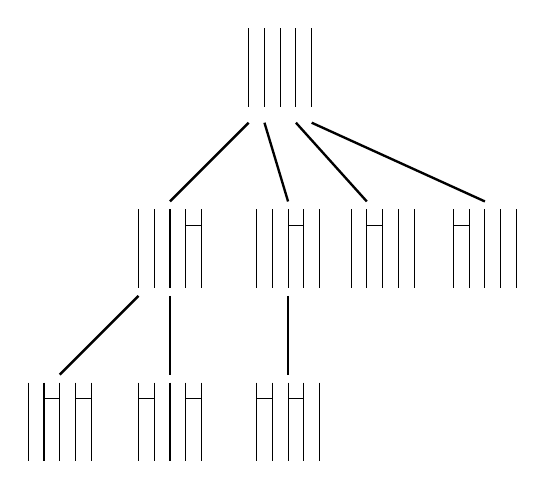
\begin{tikzpicture}
                \draw(0, 0) to (0, 1);
                \draw(.2, 0) to (.2, 1);
                \draw(.4, 0) to (.4, 1);
                \draw(.6, 0) to (.6, 1);
                \draw(.8, 0) to (.8, 1);

                \draw[line width = .3mm](0, -0.2) to (-1, -1.2);

                \draw[line width = .3mm](.2, -.2) to (.5, -1.2);

                \draw[line width = .3mm](.6, -.2) to (1.5, -1.2);
                \draw[line width = .3mm](.8, -.2) to (3, -1.2);

                \draw(-1.4, -1.3) to(-1.4, -2.3);
                \draw(-1.2, -1.3) to(-1.2, -2.3);
                \draw(-1, -1.3) to(-1, -2.3);
                \draw(-.8, -1.3) to(-.8, -2.3);
                    \draw(-.8, -1.5) to (-.6, -1.5);
                \draw(-.6, -1.3) to(-.6, -2.3);

                \draw(.1, -1.3) to (.1, -2.3);
                \draw(.3, -1.3) to (.3, -2.3);
                \draw(.5, -1.3) to (.5, -2.3);
                    \draw(.5, -1.5) to (.7, -1.5);
                \draw(.7, -1.3) to (.7, -2.3);
                \draw(.9, -1.3) to (.9, -2.3);

                \draw(1.3, -1.3) to (1.3, -2.3);
                \draw(1.5, -1.3) to (1.5, -2.3);
                    \draw(1.5, -1.5) to (1.7, -1.5);
                \draw(1.7, -1.3) to (1.7, -2.3);
                \draw(1.9, -1.3) to (1.9, -2.3);
                \draw(2.1, -1.3) to (2.1, -2.3);

                \draw(2.6, -1.3) to (2.6, -2.3);
                    \draw(2.6, -1.5) to (2.8, -1.5);
                \draw(2.8, -1.3) to (2.8, -2.3);
                \draw(3, -1.3) to (3, -2.3);
                \draw(3.2, -1.3) to (3.2, -2.3);
                \draw(3.4, -1.3) to (3.4, -2.3);

                \draw[line width = .3mm](-1.4, -2.4) to (-2.4, -3.4);
                \draw[line width = .3mm](-1, -2.4) to (-1, -3.4);
                \draw[line width = .3mm](.5, -2.4) to (.5, -3.4);
                
                \draw(-2.8, -3.5) to (-2.8, -4.5);
                \draw(-2.6, -3.5) to (-2.6, -4.5);
                    \draw(-2.6, -3.7) to (-2.4, -3.7);
                \draw(-2.4, -3.5) to (-2.4, -4.5);
                \draw(-2.2, -3.5) to (-2.2, -4.5);
                    \draw(-2.2, -3.7) to (-2, -3.7);
                \draw(-2, -3.5) to (-2, -4.5);

                \draw(-1.4, -3.5) to (-1.4, -4.5);
                    \draw(-1.4, -3.7) to (-1.2, -3.7);
                \draw(-1.2, -3.5) to (-1.2, -4.5);
                \draw(-1, -3.5) to (-1, -4.5);
                \draw(-.8, -3.5) to (-.8, -4.5);
                    \draw(-.8, -3.7) to (-.6, -3.7);
                \draw(-.6, -3.5) to (-.6, -4.5);

                 \draw(.1, -3.5) to (.1, -4.5);
                    \draw(.1, -3.7) to (.3, -3.7);
                \draw(.3, -3.5) to (.3, -4.5);
                \draw(.5, -3.5) to (.5, -4.5);
                   \draw(.5, -3.7) to (.7, -3.7);

                \draw(.7, -3.5) to (.7, -4.5);
                \draw(.9, -3.5) to (.9, -4.5);
            \end{tikzpicture}
        \end{center}
        \caption{All $7$ ladders of order $5$ with a height of one listed by the function {\sc GenHeightOne}}
        \label{Fig:GenHeightOne}
   \end{figure}

   \subsubsection{Recurrence Relation for Counting the Number of Ladders of Order $n$ with a Height of One}
   The recurrence relation of the number of ladders of order $n$ is the same recurrence relation for 
   other combinatorial objects such as the number of binary strings of length $n-1$ with no consecutive $1s$ 
   and at least one $1$~\cite{A8}\cite{A11}. The recurrence relation is used to prove the veracity of the {\sc GenHeightOne} algorithm.\par 
   
   \begin{theorem}
       The recurrence relation for the number of ladders of order $n$ with a height of $1$ is:
      \[   \left\{
        \begin{array}{ll}
        L_{count}(0) = 0 & n = 0 \\
        L_{count}(1) = 0 & n=1 \\
        L_{count}(n) = L_{count}(n-1) + L_{count}(n-2) + 1 & n \geq 2 
        \end{array} 
    \right. \]
   \end{theorem}
\begin{proof}
    We shall do a combinatorial proof to demonstrate the above theorem. 
    Suppose we want to count all binary strings of length $n$ such that there 
    can be no consecutive $1s$ and there must be at least one $1$ in the string. Suppose we are counting $1s$ from right to left. Suppose the first $1$ in a binary string of length $n$ is at position $n$, 
    then the second $1$ can appear at position $n-2$, thus we have binary 
    strings of length $n$ with the first $1$ appearing at position $n$ and the second one appearing at position $n-2$; 
    let $m=$ the number of binary strings of length $n$ such that there is a $1$ 
    at position $n-2$. Next, suppose a binary string of length $n$ has a $0$ at position $n$, then
    the first $1$ can appear at position $n-1$ or position $n-2$. 
    If it appears at position $n-2$ we have binary strings of length $n$ with a $1$ at position $n-2$. 
    We already designated this number as $m$, so we get $2(m)$. 
    Still supposing we are considering binary strings of length $n$ with a $0$ at position $n$, consider all binary strings of length $n-1$ with 
    no consecutive $1s$. Let $k=$ the number of binary strings of length $n-1$ with no consecutive $1s$ and at least one $1$.
    Let the first $1$ in the binary string of length $n$ appears at position $n-1$, then we have $2(m)+k$. 
    Still assuming a $0$ at position $n$
    in binary strings of length $n$, if there is also a $0$ at position $n-1$, then the first $1$ can appear at position $n-2$. 
    The number of 
    binary strings of length $n$ with a $1$ at position $n$ was designated as $m$. 
    Thus we have $2(m)+m=3m$
    Yet we have already counted $m$ 
    under the conditions that the first $1$ in binary strings of length $n$ appears at position $n-2$. 
    Therefore we subtract 
    $m$ from $k$ thus leaving us with $j=$ the number of binary strings of length $n$ with the first $1$ appearing at position $n-1$. 
    Now we have $2(m)+j$. T
    hen consider all binary strings of length $n$ such that from positions $1\dots n-1$ there are 
    only $0s$. Therefore, there must be a $1$ at position $n$ seeing as we are considering all binary strings of length $n$ with at least one $1$. 
    Only one such binary string of length $n$ exists, therefore we add one. We get $2(m)+(k-m)+1=2(m)+j+1=$ 
    the number of binary strings of length $n$ with at least one $1$ and 
    no consecutive $1s$.\par 
    Now consider a ladder, $L$, with $n+1$ lines. The number of columns in $L$ is $n$ and the height of $L$ is one. Note that the end points 
    of no two bars can be touching which is to say that there can be no adjacent bars on the same row. For example, 
    if there is a bar at row $1$, column $n$ then 
    the next consecutive bar in row $1$ can appear at most at column $n-2$. 
    Knowing this, we can easily see how this scenario models all binary strings of length $n$ with no 
    consecutive $1s$ and having at least one $1$. Let a bar in $l$ be represented as a $1$ in a binary string of length $n$. 
    Knowing that a ladder with zero bars has a height of zero, it must be the case that $l$ has at least one bar. 
    Thus, we get the same recurrence relation for the number of 
    ladders of order $n+1$ where $m$ is the number of ladders with a bar appearing in column $n-2$, $(k-m)=j$ 
    being the number of ladders with the first bar in column $n-1$ minus 
    ladders with a bar appearing at $n-2$. Lastly is the $+1$ for all ladders of order $n+1$ where the only bar appears at column $n$.
    See Figure~\ref{Fig:MapBinToLadder} for the mapping of binary strings of length $n=5$ with no consecutive $1s$ and at 
    least one $1$ to ladders of order $6$ with a height of one.\pagebreak

\end{proof}

\begin{center}
    
\begin{figure}[!htp]
    \begin{minipage}{.4\textwidth}

    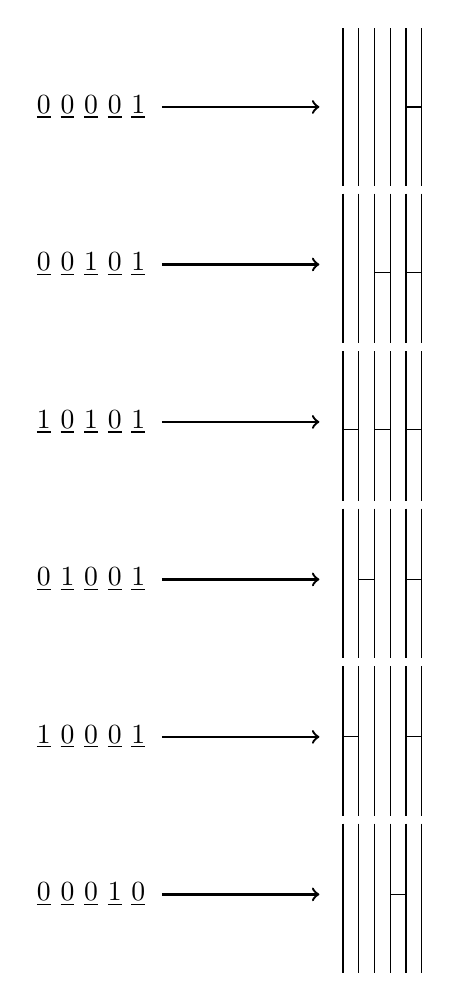
\begin{tikzpicture}
            
        
            
        %%B1
        \node at(0, 0){\underline{$0$}};
        \node at(0.3, 0){\underline{$0$}};
        \node at(0.6, 0){\underline{$0$}};
        \node at(0.9, 0){\underline{$0$}};
        \node at(1.2, 0){\underline{$1$}};
            \draw[->, line width = .3mm](1.5, 0) to (3.5, 0);
        %%L1
        \draw(3.8, -1) to (3.8, 1);
        \draw(4, -1) to (4, 1);
        \draw(4.2, -1) to (4.2, 1);
        \draw(4.4, -1) to (4.4, 1);
            \draw(4.6, 0) to (4.8, 0);
        \draw(4.6, -1) to (4.6, 1);
        \draw(4.8, -1) to (4.8, 1);
        %B2
        \node at (0, -2){\underline{$0$}};
        \node at (.3, -2){\underline{$0$}};
        \node at (.6, -2){\underline{$1$}};
        \node at (.9, -2){\underline{$0$}};
        \node at (1.2, -2){\underline{$1$}};
            \draw[->, line width = .3mm](1.5, -2) to (3.5, -2);

        %%L2
        \draw(3.8, -1.1) to (3.8, -3);
        \draw(4, -1.1) to (4, -3);
        \draw(4.2, -1.1) to (4.2, -3);
        \draw(4.4, -1.1) to (4.4, -3);
            \draw(4.6, -2.1) to (4.8, -2.1);
            \draw(4.2, -2.1) to (4.4, -2.1);
        \draw(4.6, -1.1) to (4.6, -3);
        \draw(4.8, -1.1) to (4.8, -3);

        %%B3
        \node at (0, -4){\underline{$1$}};
        \node at (.3, -4){\underline{$0$}};
        \node at (.6, -4){\underline{$1$}};
        \node at (.9, -4){\underline{$0$}};
        \node at (1.2, -4){\underline{$1$}};
                    \draw[->, line width = .3mm](1.5, -4) to (3.5, -4);

        %%L3
        \draw(3.8, -3.1) to (3.8, -5);
        \draw(4, -3.1) to (4, -5);
        \draw(4.2, -3.1) to (4.2, -5);
        \draw(4.4, -3.1) to (4.4, -5);
            \draw(4.6, -4.1) to (4.8, -4.1);
            \draw(4.2, -4.1) to (4.4, -4.1);
            \draw(3.8, -4.1) to (4, -4.1);
        \draw(4.6, -3.1) to (4.6, -5);
        \draw(4.8, -3.1) to (4.8, -5);
    
        %%B4
        \node at (0, -6){\underline{$0$}};
        \node at (.3, -6){\underline{$1$}};
        \node at (.6, -6){\underline{$0$}};
        \node at (.9, -6){\underline{$0$}};
        \node at (1.2, -6){\underline{$1$}};

        \draw[->, line width=.3mm](1.5, -6) to (3.5, -6);
        %%L4
        \draw(3.8, -5.1) to (3.8, -7);
        \draw(4, -5.1) to (4, -7);
            \draw(4, -6) to (4.2, -6);
        \draw(4.2, -5.1) to (4.2, -7);
        \draw(4.4, -5.1) to (4.4, -7);
        \draw(4.6, -5.1) to (4.6, -7);
            \draw(4.6, -6) to (4.8, -6);
        \draw(4.8, -5.1) to (4.8, -7);

        %%B5
        \node at (0, -8){\underline{$1$}};
        \node at (.3, -8){\underline{$0$}};
        \node at (.6, -8){\underline{$0$}};
        \node at (.9, -8){\underline{$0$}};
        \node at (1.2, -8){\underline{$1$}};

            \draw[->, line width=.3mm](1.5, -8) to (3.5, -8);
        %%L5
        \draw(3.8, -7.1) to (3.8, -9);
        \draw(4, -7.1) to (4, -9);
            \draw(3.8, -8) to (4, -8);
        \draw(4.2, -7.1) to (4.2, -9);
        \draw(4.4, -7.1) to (4.4, -9);
        \draw(4.6, -7.1) to (4.6, -9);
            \draw(4.6, -8) to (4.8, -8);
        \draw(4.8, -7.1) to (4.8, -9);

         %%B6
        \node at (0, -10){\underline{$0$}};
        \node at (.3, -10){\underline{$0$}};
        \node at (.6, -10){\underline{$0$}};
        \node at (.9, -10){\underline{$1$}};
        \node at (1.2, -10){\underline{$0$}};

            \draw[->, line width=.3mm](1.5, -10) to (3.5, -10);
        %%L6
        \draw(3.8, -9.1) to (3.8, -11);
        \draw(4, -9.1) to (4, -11);
        \draw(4.2, -9.1) to (4.2, -11);
        \draw(4.4, -9.1) to (4.4, -11);
            \draw(4.4, -10) to (4.6, -10);
        \draw(4.6, -9.1) to (4.6, -11);
        \draw(4.8, -9.1) to (4.8, -11);

    \end{tikzpicture}
    \end{minipage}
    \begin{minipage}{.4\textwidth}
        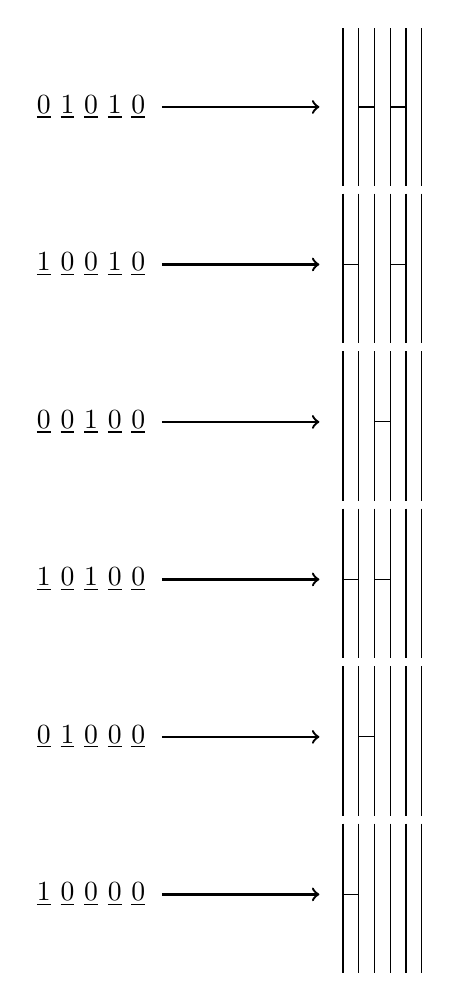
\begin{tikzpicture}
          %%B7
        \node at(0, 0){\underline{$0$}};
        \node at(0.3, 0){\underline{$1$}};
        \node at(0.6, 0){\underline{$0$}};
        \node at(0.9, 0){\underline{$1$}};
        \node at(1.2, 0){\underline{$0$}};
            \draw[->, line width = .3mm](1.5, 0) to (3.5, 0);
        %%L7
        \draw(3.8, -1) to (3.8, 1);
        \draw(4, -1) to (4, 1);
        \draw(4.2, -1) to (4.2, 1);
            \draw(4, 0) to (4.2, 0);
        \draw(4.4, -1) to (4.4, 1);
            \draw(4.4, 0) to (4.6, 0);
        \draw(4.6, -1) to (4.6, 1);
        \draw(4.8, -1) to (4.8, 1);


        %%B8
        \node at(0, -2){\underline{$1$}};
        \node at(0.3, -2){\underline{$0$}};
        \node at(0.6, -2){\underline{$0$}};
        \node at(0.9, -2){\underline{$1$}};
        \node at(1.2, -2){\underline{$0$}};
            \draw[->, line width = .3mm](1.5, -2) to (3.5, -2);
        %%L8
        \draw(3.8, -1.1) to (3.8, -3);
        \draw(4, -1.1) to (4, -3);
        \draw(4.2, -1.1) to (4.2, -3);
            \draw(3.8, -2) to (4, -2);
        \draw(4.4, -1.1) to (4.4, -3);
            \draw(4.4, -2) to (4.6, -2);
        \draw(4.6, -1.1) to (4.6, -3);
        \draw(4.8, -1.1) to (4.8, -3);


         %%B9
        \node at(0, -4){\underline{$0$}};
        \node at(0.3, -4){\underline{$0$}};
        \node at(0.6, -4){\underline{$1$}};
        \node at(0.9, -4){\underline{$0$}};
        \node at(1.2, -4){\underline{$0$}};
            \draw[->, line width = .3mm](1.5, -4) to (3.5, -4);
        %%L9
        \draw(3.8, -3.1) to (3.8, -5);
        \draw(4, -3.1) to (4, -5);
        \draw(4.2, -3.1) to (4.2, -5);
            \draw(4.2, -4) to (4.4, -4);
        \draw(4.4, -3.1) to (4.4, -5);
        \draw(4.6, -3.1) to (4.6, -5);
        \draw(4.8, -3.1) to (4.8, -5);


        
         %%B10
        \node at(0, -6){\underline{$1$}};
        \node at(0.3, -6){\underline{$0$}};
        \node at(0.6, -6){\underline{$1$}};
        \node at(0.9, -6){\underline{$0$}};
        \node at(1.2, -6){\underline{$0$}};
            \draw[->, line width = .3mm](1.5, -6) to (3.5, -6);
        %%L10
        \draw(3.8, -5.1) to (3.8, -7);
            \draw(3.8, -6) to (4,-6);
        \draw(4, -5.1) to (4, -7);
        \draw(4.2, -5.1) to (4.2, -7);
            \draw(4.2, -6) to (4.4, -6);
        \draw(4.4, -5.1) to (4.4, -7);
        \draw(4.6, -5.1) to (4.6, -7);
        \draw(4.8, -5.1) to (4.8, -7);

        %%B1
        \node at(0, -8){\underline{$0$}};
        \node at(0.3, -8){\underline{$1$}};
        \node at(0.6, -8){\underline{$0$}};
        \node at(0.9, -8){\underline{$0$}};
        \node at(1.2, -8){\underline{$0$}};
            \draw[->, line width = .3mm](1.5, -8) to (3.5, -8);
        %%L11
        \draw(3.8, -7.1) to (3.8, -9);
        \draw(4, -7.1) to (4, -9);
            \draw(4, -8) to (4.2, -8);
        \draw(4.2, -7.1) to (4.2, -9);
        \draw(4.4, -7.1) to (4.4, -9);
        \draw(4.6, -7.1) to (4.6, -9);
        \draw(4.8, -7.1) to (4.8, -9);

         %%B12
        \node at(0, -10){\underline{$1$}};
        \node at(0.3, -10){\underline{$0$}};
        \node at(0.6, -10){\underline{$0$}};
        \node at(0.9, -10){\underline{$0$}};
        \node at(1.2, -10){\underline{$0$}};
            \draw[->, line width = .3mm](1.5, -10) to (3.5, -10);
        %%L12
        \draw(3.8, -9.1) to (3.8, -11);
            \draw(3.8, -10) to (4, -10);
        \draw(4, -9.1) to (4, -11);
        \draw(4.2, -9.1) to (4.2, -11);
        \draw(4.4, -9.1) to (4.4, -11);
        \draw(4.6, -9.1) to (4.6, -11);
        \draw(4.8, -9.1) to (4.8, -11);
        \end{tikzpicture}
    \end{minipage}

    \caption{All 12 binary strings of length $5$ with at least one $1$ and no consecutive $1s$ maps to all twelve ladders of order $6$ with a height of one. 
    The recurrence relation being $L(6)=2L(4)+(L(5)-L(4))+1=L(4)+L(5)+1$}
    \label{Fig:MapBinToLadder}
\end{figure}
\end{center}



\subsubsection{Closed form Formula for Ladders of Order $n$ with a Height of One}
Before providing the closed form formula for the number of ladders with a height of one, it is important to connect ladders with a height of one 
to other mathematical phenomena because ladders with a height follow the same pattern as these other mathematical phenomena~\cite{A12}.
One of these phenomena include the number of involutions in the Symmetric Group $S_{n}$~\cite{A13}. 
The connection between the Symmetric Group, $S_{n}$ and ladders of order $n$ with a height 
of zero or one will be analyzed followed by the closed form formula.\par 

A \emph{group} is a finite set along with a binary operation on the elements of the set such that the binary operation on two 
elements in the set produces a result that is also in the set. 
The stipulations of a group are the following. Firstly, the group must have \emph{closure} which means the 
result of the binary operation produces a result in the set; this stipulation was already addressed in the definition of a group. 
Secondly, the group must 
be associative, meaning the rearrangement of priority of the order of application of the binary operation across $2 \leq k$ $\leq n$ 
elements in the set 
does not change the result; associativity means the order of application of the binary operation across multiple elements in the set does 
not change the result. The third stipulation 
is that the set has the identity element. 
The identity element is the element such that when the binary operation is applied to an element, $x$, with the identity element
the result is $x$. The fourth stipulation is the \emph{inverse element} 
which is a relation between two elements, $x$ and $y$ such that when the binary operation is applied to $x$ and 
its inverse element $y$, 
the result is $x$~\cite{A14}.\par 

A \emph{symmetric group of order $n$/$S_{n}$} is finite group whose elements are all $n!$ permutations of order $n$, the binary operation 
is permutation composition, applying the composition forms a bijection between all elements in the set. When a permutation is written in 
cycle notation, the \emph{orbit} is defined as the transposition of elements on the identity permutation. For example, 
let $\pi=(3,2,1,6,4,5,7)$ be written as $(1,3)(4,5,6)$ in cycle notation. There are two orbits, one of size two, namely $(1,3)$ and 
one of size three, namely $(4,5,6)$~\cite{A15}. There Let an \emph{involution} 
be defined as a composition of a permutation with itself such that the result of the composition is the identity permutation~\cite{A13}. 
For example, $X=\{1, 2, 3\}$. Let $S_{X} = S_{n} = \{(1,2,3),(1,3,2),(2,1,3),(2,3,1),(3,1,2),(3,2,1)\}$. 
The involutions of $S_{n}=\{(2,1,3),(1,3,2),(1,2,3)\}$.
The reason these are the involutions is because when we define a permutation as a bijective function on the identity permutation, 
we can see the the composition 
of an involution with itself returns the identity permutation. Let $(1,2,3)=F$, let $(2,1,3)=G$ and let $(1,3,2)=H$ 
then we have $F \circ F=(1,2,3)$,
$G \circ G = (1,2,3)$ and 
$H \circ H=(1,2,3)$. The orbit(s) of an involution are of size two and 
the orbits are transitive, meaning the elements composing the orbit(s) are adjacent in the identity permutation.
To see an example of the mapping of the composition of $(2,1,3)$ with itself see Figure~\ref{Fig:InvolutionExample}\newline 


\begin{figure}
 \centering
 \begin{tikzpicture}[ele/.style={fill=black,circle,minimum width=.8pt,inner sep=1pt},every fit/.style={ellipse,draw,inner sep=-2pt}]
  \node[ele,label=left:$1$] (a1) at (0,4) {};    
  \node[ele,label=left:$2$] (a2) at (0,3) {};    
  \node[ele,label=left:$3$] (a3) at (0,2) {};

  \node[ele,,label=right:$1$] (b1) at (4,4) {};
  \node[ele,,label=right:$2$] (b2) at (4,3) {};
  \node[ele,,label=right:$3$] (b3) at (4,2) {};

  \node [ele,,label=right:$1$](c1) at (8,4){};
  \node [ele,,label=right:$2$](c2) at (8,3){};
  \node [ele,,label=right:$3$](c3) at (8,2){};
  \node[draw,fit= (a1) (a2) (a3),minimum width=2cm] {} ;
  \node[draw,fit= (b1) (b2) (b3), minimum width=2cm] {} ;  
  \node[draw,fit= (c1) (c2) (c3), minimum width=2cm] {} ;  

  \draw[->,thick,shorten <=2pt,shorten >=2pt] (a1) -- (b2);
  \draw[->,thick,shorten <=2pt,shorten >=2] (a2) -- (b1);
  \draw[->,thick,shorten <=2pt,shorten >=2] (a3) -- (b3);
  \draw[->,thick,shorten <=0pt,shorten >=0pt] (b1) -- (c2);
  \draw[->,thick,shorten <=1pt,shorten >=2pt] (b2) -- (c1);
  \draw[->,thick,shorten <=1pt,shorten >=2pt] (b3) -- (c3);

  \node at (2,4.5){$G(1,2,3)$};
  \node at(6,4.5){$G \circ G(1,2,3)$};
   \node at(-3, 3){\small{$G=(2,1,3)$}};
 \end{tikzpicture}
 
 \caption{The involution $(2,1,3)$ composed with itself when applied to the identity permutation returns the identity permutation}
 \label{Fig:InvolutionExample}
\end{figure}

\begin{theorem}
    There is a bijective function between ladders of order $n$ with a height of zero or one and the involution set of $S_{n}$.
\end{theorem}
\begin{proof}
    The involution set of $S_{n}$ consists of all permutations of order $n$ 
    such that when any permutation is composed with itself, the result of the composition is the identity permutation. 
    If a permutation is an involution then it either has no inversions or for each pair of inversions, the inversion pairs are pairwise disjoint. 
    That is to say, no element in the 
    permutation forms more than $1$ inversion. 
    When an involution is applied to the identity permutation, each element in the identity is 
    rotated by one or zero positions. 
    If an element from the identity permutation is rotated two times over over a span of two positions, 
    the element returns to its original position in the identity permutation.
    Thus, applying an involution to itself either rotates an element zero times or it rotates an element twice over a span of two positions, 
    thus placing the element in its 
    original position in the identity permutation.\par 
    A ladder of order $n$ with a height of one consists only of bars such that no element crosses more than one of these bars. 
    Suppose an element $x$
    needed to be cross more than one bar. This would mean the route of $x>1$. If that is the case then the height of the ladder would 
    be greater than one, which contradicts the claim that the ladder has a height of one.
    Then it must be the case that for all ladders of order $n$ with a height of one, each bar in any of these given ladders 
    uninverts a pair of elements in $\pi$ exactly once and no two bars 
    have the same element crossing them. It follows that each bar places an element in $\pi$ to its correct position 
    in the identity permutation.  
    We know that each ladder with a height of zero or one is unique, in that they all sort different permutations,
    because the only way to get 
    two or more ladders to sort the same permutation is to perform a swap operation on bar(s) in a ladder to get 
    another ladder in $OptL\{\pi\}$.
    Yet with ladders of height zero or one, no swap operation can be performed.\par
    Let $F(L_{n})$ be the representation of a ladder as a function. We have already established that an 
    involution can be thought of as a function. Let $G$ be the representation of an 
    involution as a function. We know that $G \circ G(\pi_{ID})=\pi_{ID}$. I propose that for each $G$ there is a corresponding $F(L_{n})$
    such that $F(L_{n}) \circ G(\pi_{ID}) = \pi_{ID}$ where each $F(L_{n})$ and $G$ are unique. 
    This shall be proven by way of contradiction. Suppose there exists a $G$ of order $n$ such that  $F(L_{n}) \circ G(\pi_{ID}) \neq \pi_{ID}$ 
    for every $F(L_{n})$.
    Let this $G$ be known as $k$. 
    We know that the number of ladders with a height of zero or one of order $n$ equals the number of involutions of order $n$. 
    We also know that each bar in $F(L_{n})$ of order one uninverts an inversion in $\pi$ 
    We know that each $G$ is unique seeing as the involution set $\subset$ all $n!$ permutations and all 
    $n!$ permutations are unique. Thus, if $F(L_{n}) \circ K(\pi_{ID}) \neq \pi_{ID}$ for every $F(L_{n})$ 
    of a height of zero or one that means either there is a 
    $F(L_{n})$ of height zero or one that does not map $K$ to $pi_{ID}$ when composed with $K$ or there exists at least two $F(L_{n})$ 
    of height zero or one that map the 
    same $G \neq K$ to $\pi_{ID}$ when composed with $G$. 
    In the first case this would mean that there is some involution, $K$, that could not be sorted into the identity 
    permutation by any $F(L_{n})$ of height zero or one. Yet if that is the case then there is an $F(L_{n})$ 
    of height zero or one such that there exists 
    a bar in $F(L_{n})$ that does not place the element crossing it into its correct position in $ID$. 
    But if that is the case then $F(L_{n})$ does not 
    have a height of zero or one which is a contradiction. 
    In the second case, this would mean that there are two $F(L_{n})$ with a height of zero or one, 
    let us call them $A$ and $B$, and some $G\neq K$, such that $A\circ G(\pi_{ID}) = B\circ G(\pi_{ID})=\pi_{ID}$ and $A \neq B$. 
    Yet we know that the only way for two unique ladders 
    to sort the same permutation is by right/left swapping the bars of one ladder to get the configuration of the bars in the other ladder. 
    Yet a bar cannot be 
    right/left swapped in a ladder with a height of zero or one. Thus, if 
    $A\circ G(\pi_{ID}) = B\circ G(\pi_{ID})=\pi_{ID}$ it must be the case that $A=B$ which is a contradiction. Therefore, 
    for each $G$ there exists an $F(L_{n})$ such that 
     $F(L_{n}) \circ G(\pi_{ID}) = \pi_{ID}$ where each $F(L_{n})$ and $G$ are unique. 
     To see the bijective mapping 
     between ladders of order $4$ with a height of zero or one and the involution set of $S_{4}$ please refer to Figure~\ref{Fig:BijectiveMapping}.
\end{proof}\pagebreak
\begin{figure}[ht]
    \centering
        \begin{tikzpicture}[ele/.style={fill=black,circle,minimum width=.8pt,inner sep=1pt},every fit/.style={ellipse,draw,inner sep=-1pt}]
        %%1
        \node at(1.5, .5){$G=()$};
        \node at(-.5, .5){$L=$};
        \draw(0, 0) to (0, 1);
        \draw(.2, 0) to (.2, 1);
        \draw(.4, 0) to (.4, 1);
        \draw(.6, 0) to (.6, 1);

        \node[ele,label=left:$1$] (a1) at (6,1.2) {};    
        \node[ele,label=left:$2$] (a2) at (6,.7) {};    
        \node[ele,label=left:$3$] (a3) at (6,.2) {};
        \node[ele,label=left:$4$] (a4) at (6,-.3) {};
        \node[draw,fit= (a1) (a2) (a3) (a4), minimum width=2cm] {} ;  

         \node[ele,label=left:$1$] (b1) at (9,1.2) {};    
        \node[ele,label=left:$2$] (b2) at (9,.7) {};    
        \node[ele,label=left:$3$] (b3) at (9,.2) {};
        \node[ele,label=left:$4$] (b4) at (9,-.3) {};
        \node[draw,fit= (b1) (b2) (b3) (b4), minimum width=2cm] {} ;  
 
        \node[ele,label=right:$1$] (c1) at (12,1.2) {};    
        \node[ele,label=right:$2$] (c2) at (12,.7) {};    
        \node[ele,label=right:$3$] (c3) at (12,.2) {};
        \node[ele,label=right:$4$] (c4) at (12,-.3) {};
        \node[draw,fit= (c1) (c2) (c3) (c4), minimum width=2cm] {} ;  

        \draw[->,thick,shorten <=1pt,shorten >=1pt] (a1) -> (b1) ->(c1);
        \draw[->,thick,shorten <=2pt,shorten >=2pt] (a2) -> (b2) -> (c2);
        \draw[->,thick,shorten <=2pt,shorten >=2pt] (a3) -> (b3) -> (c3);
        \draw[->,thick,shorten <=2pt,shorten >=2pt] (a4) -> (b4) -> (c4);




        %%2
        \node at(2, 3.5){$G=(1,2)$};
        \node at(-.5, 3.5){$L=$};
        \draw(0, 3) to (0, 4);
            \draw(0, 3.5) to (.2, 3.5);
        \draw(.2, 3) to (.2, 4);
        \draw(.4, 3) to (.4, 4);
        \draw(.6, 3) to (.6, 4);

        \node[ele,label=left:$1$] (d1) at (6,4.2) {};    
        \node[ele,label=left:$2$] (d2) at (6,3.7) {};    
        \node[ele,label=left:$3$] (d3) at (6,3.2) {};
        \node[ele,label=left:$4$] (d4) at (6,2.7) {};
        \node[draw,fit= (d1) (d2) (d3) (d4), minimum width=2cm] {} ;  

         \node[ele,label=left:$1$] (e1) at (9,4.2) {};    
        \node[ele,label=left:$2$] (e2) at (9,3.7) {};    
        \node[ele,label=left:$3$] (e3) at (9,3.2) {};
        \node[ele,label=left:$4$] (e4) at (9,2.7) {};
        \node[draw,fit= (e1) (e2) (e3) (e4), minimum width=2cm] {} ;  
 
        \node[ele,label=right:$1$] (f1) at (12,4.2) {};    
        \node[ele,label=right:$2$] (f2) at (12,3.7) {};    
        \node[ele,label=right:$3$] (f3) at (12,3.2) {};
        \node[ele,label=right:$4$] (f4) at (12,2.7) {};
        \node[draw,fit= (f1) (f2) (f3) (f4), minimum width=2cm] {} ;  


        \draw[->,thick,shorten <=1pt,shorten >=1pt] (d1) -> (e2) ->(f1);
        \draw[->,thick,shorten <=2pt,shorten >=2pt] (d2) -> (e1) -> (f2);
        \draw[->,thick,shorten <=2pt,shorten >=2pt] (d3) -> (e3) -> (f3);
        \draw[->,thick,shorten <=2pt,shorten >=2pt] (d4) -> (e4) -> (f4);

        %%3
        \node at(2, 6.5){$G=(2,3)$};
        \node at(-.5, 6.5){$L=$};
        \draw(0, 6) to (0, 7);
        \draw(.2, 6) to (.2, 7);
            \draw(.2, 6.5) to (.4, 6.5);
        \draw(.4, 6) to (.4, 7);
        \draw(.6, 6) to (.6, 7);


        \node[ele,label=left:$1$] (g1) at (6,7.2) {};    
        \node[ele,label=left:$2$] (g2) at (6,6.7) {};    
        \node[ele,label=left:$3$] (g3) at (6,6.2) {};
        \node[ele,label=left:$4$] (g4) at (6,5.7) {};
        \node[draw,fit= (g1) (g2) (g3) (g4), minimum width=2cm] {} ;  

         \node[ele,label=left:$1$] (h1) at (9,7.2) {};    
        \node[ele,label=left:$2$] (h2) at (9,6.7) {};    
        \node[ele,label=left:$3$] (h3) at (9,6.2) {};
        \node[ele,label=left:$4$] (h4) at (9,5.7) {};
        \node[draw,fit= (h1) (h2) (h3) (h4), minimum width=2cm] {} ;  
 
        \node[ele,label=right:$1$] (i1) at (12,7.2) {};    
        \node[ele,label=right:$2$] (i2) at (12,6.7) {};    
        \node[ele,label=right:$3$] (i3) at (12,6.2) {};
        \node[ele,label=right:$4$] (i4) at (12,5.7) {};
        \node[draw,fit= (i1) (i2) (i3) (i4), minimum width=2cm] {} ;  

        \draw[->,thick,shorten <=1pt,shorten >=1pt] (g1) -> (h1) ->(i1);
        \draw[->,thick,shorten <=2pt,shorten >=2pt] (g2) -> (h3) -> (i2);
        \draw[->,thick,shorten <=2pt,shorten >=2pt] (g3) -> (h2) -> (i3);
        \draw[->,thick,shorten <=2pt,shorten >=2pt] (g4) -> (h4) -> (i4);

        

        %%4
        \node at(2, 9.5){$G=(3,4)$};
        \node at(-.5, 9.5){$L=$};
        \draw(0, 9) to (0, 10);
        \draw(.2, 9) to (.2, 10);
        \draw(.4, 9) to (.4, 10);
            \draw(.4, 9.5) to (.6, 9.5);
        \draw(.6, 9) to (.6, 10);


       \node[ele,label=left:$1$] (j1) at (6,10.2) {};    
        \node[ele,label=left:$2$] (j2) at (6,9.7) {};    
        \node[ele,label=left:$3$] (j3) at (6,9.2) {};
        \node[ele,label=left:$4$] (j4) at (6,8.7) {};
        \node[draw,fit= (j1) (j2) (j3) (j4), minimum width=2cm] {} ;  

         \node[ele,label=left:$1$] (k1) at (9,10.2) {};    
        \node[ele,label=left:$2$] (k2) at (9,9.7) {};    
        \node[ele,label=left:$3$] (k3) at (9,9.2) {};
        \node[ele,label=left:$4$] (k4) at (9,8.7) {};
        \node[draw,fit= (k1) (k2) (k3) (k4), minimum width=2cm] {} ;  
 
        \node[ele,label=right:$1$] (l1) at (12,10.2) {};    
        \node[ele,label=right:$2$] (l2) at (12,9.7) {};    
        \node[ele,label=right:$3$] (l3) at (12,9.2) {};
        \node[ele,label=right:$4$] (l4) at (12,8.7) {};
        \node[draw,fit= (l1) (l2) (l3) (l4), minimum width=2cm] {} ;  

        \draw[->,thick,shorten <=1pt,shorten >=1pt] (j1) -> (k1) ->(l1);
        \draw[->,thick,shorten <=2pt,shorten >=2pt] (j2) -> (k2) -> (l2);
        \draw[->,thick,shorten <=2pt,shorten >=2pt] (j3) -> (k4) -> (l3);
        \draw[->,thick,shorten <=2pt,shorten >=2pt] (j4) -> (k3) -> (l4);


        

        %%5
        \node at(2.5, 12.5){$G=(1,2)(3,4)$};
        \node at(-.5, 12.5){$L=$};
        \draw(0, 12) to (0, 13);
            \draw(0, 12.5) to (.2, 12.5);
            \draw(.4, 12.5) to (.6, 12.5);
        \draw(.2, 12) to (.2, 13);
        \draw(.4, 12) to (.4, 13);
        \draw(.6, 12) to (.6, 13);

        \node[ele,label=left:$1$] (m1) at (6,13.2) {};    
        \node[ele,label=left:$2$] (m2) at (6,12.7) {};    
        \node[ele,label=left:$3$] (m3) at (6,12.2) {};
        \node[ele,label=left:$4$] (m4) at (6,11.7) {};
        \node[draw,fit= (m1) (m2) (m3) (m4), minimum width=2cm] {} ;  

         \node[ele,label=left:$1$] (n1) at (9,13.2) {};    
        \node[ele,label=left:$2$] (n2) at (9,12.7) {};    
        \node[ele,label=left:$3$] (n3) at (9,12.2) {};
        \node[ele,label=left:$4$] (n4) at (9,11.7) {};
        \node[draw,fit= (n1) (n2) (n3) (n4), minimum width=2cm] {} ;  
 
        \node[ele,label=right:$1$] (o1) at (12,13.2) {};    
        \node[ele,label=right:$2$] (o2) at (12,12.7) {};    
        \node[ele,label=right:$3$] (o3) at (12,12.2) {};
        \node[ele,label=right:$4$] (o4) at (12,11.7) {};
        \node[draw,fit= (o1) (o2) (o3) (o4), minimum width=2cm] {} ;  


        \draw[->,thick,shorten <=1pt,shorten >=1pt] (m1) -> (n2) ->(o1);
        \draw[->,thick,shorten <=2pt,shorten >=2pt] (m2) -> (n1) -> (o2);
        \draw[->,thick,shorten <=2pt,shorten >=2pt] (m3) -> (n4) -> (o3);
        \draw[->,thick,shorten <=2pt,shorten >=2pt] (m4) -> (n3) -> (o4);


        \node at(7.5, 14){\small{$G(1,2,3,4)$}};
        \node at(10.6, 14){\small{$L \circ G(1,2,3,4)$}};

    
        \end{tikzpicture}
        \caption{All ladders of order $4$ with a height of zero or one form a bijection with the involution set of $S_{4}$.}
        \label{Fig:BijectiveMapping}
\end{figure}
\pagebreak
So far we have demonstrated that ladders of order $n$ with a height of one are congruent with binary strings of length $n-1$ 
with no consecutive ones and at least one $1$ and the involution set of $S_{n}$. The final mathematical phenomena to be discussed 
is the \emph{Fibonacci sequence}. The Fibonacci sequence is the sequence $0,1,1,2,3,5,8,13, \dots$. It is defined by the
recurrence relation:\cite{A12}

 \[   
     \left\{
       \begin{array}{ll}
        Fib(0) = 0 & n = 0 \\
        Fib(1) = 1 & n=1 \\
        Fib(n) = Fib(n-1) + Fib(n-2) & n \geq 2 
        \end{array} 
    \right.
\]


The Fibonacci sequence is considered famous for its occurrence in natural phenomena such as the structure of a pine cone, the number of petals 
on sunflowers and the spiral of the shells of ammonites which are a prehistoric crustaceans. The Fibonacci sequence was first discovered by an 
Indian mathematician named Pingala at some time between 450 - 200 BCE~\cite{A16}. It was then introduced to Western cultures in 1202 by the 
Italian mathematician, Fibonacci. The recurrence relation for the Fibonacci numbers should look familiar to the recurrence 
relation for the number of ladders of order $n$ with a height of one. The difference between the two is the recurrence relation 
for the number of ladders of order $n$ with a height of one has an additional $+1$ because of the single ladder of 
order $n$ in which the first $n-2$ columns have a $0$ in row one and the last column has a $1$ in row one. Other than the additional 
$+1$, the sequences are the same. Please refer to Figure~\ref{Fig:FibLadderSequence} to see the sequences together.\newline
    
\begin{figure}[!htp]
    \centering
    $Fib: \qquad 00,01,01,02,03,05,08,13,21,34,55, \dots$\newline
    $L_{count}: \quad   00,00,01,02,04,07,12,20,33,54,88, \dots$\newline
    $n: \qquad   00,01,02,03,04,05,06,07,08,09,10, \dots$\newline
    \caption{The Fibonacci sequence lined up with the sequence for the number of ladders with a height of one.}
    \label{Fig:FibLadderSequence}

\end{figure}

From looking at the sequences in Figure~\ref{Fig:FibLadderSequence}, it is interesting to note that\newline
$L_{count}(n)=Fib(n+1)-1$. 
There is a well known equation for the Fibonacci sequence which is the following: 

\begin{equation*}
   Fib(n)=1/\sqrt{5}((1+\sqrt{5}/2)^{n})((1-\sqrt{5}/2)^{n}))
\end{equation*}\cite{A12}
From the Fibonacci equation along with the equation $L_{count}(n)=Fib(n+1)-1$, it is fairly straightforward to derive the 
equation for $L_{count}(n)$
\begin{center}
\begin{equation*}
    L_{count}(n)=1/\sqrt{5} ((1+\sqrt{5}/2)^{n+1})((1-\sqrt{5}/2)^{n+1}))-1
\end{equation*}
\end{center}
The equation is simply the closed form formula for the $n+1th$ Fibonacci number minus $1$.\par 

We have examined the congruence between ladders of a height of one with three other mathematical phenomena. The three being 
binary strings of length $n-1$ with at least one $1$ and no consecutive $1s$, the involution set of the symmetric group $S_{n}$
and the Fibonacci sequence. The similarities between these mathematical phenomena is of theoretical interest because it has been 
shown that the set containing all mathematical phenomena that follow the sequence $0,0,1,2,4,7,12,20\dots$ also contains 
ladders with a height of one.




%%End section with ladders of a height of zero or one